%!TEX root =../mapp-challenge-18-game-book.tex
% ^ leave for LaTeXTools build functionality

\phChapterWorksheet{The Expedition Zone}{Bonus Puzzle}

Take a trip through the \textbf{Expedition Zone} to catch as many Mobimon as you
can! Theres a catch, though: your path through the Expedition Zone has to follow
certain \textbf{expedition pieces.} Here are the rules:
\begin{enumerate}
\item Two expedition pieces are adjacent if any of their \textbf{corners} are
  touching, but \textbf{no other parts touch}.
  \begin{center}
    These pieces are adjacent.

    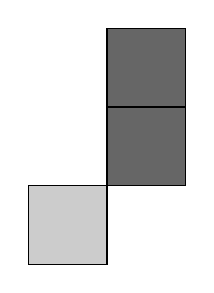
\begin{tikzpicture}
      \draw[fill=black!20] (0,0) grid (1,1) rectangle (0,0);
      \draw[fill=black!60] (1,1) grid (2,3) rectangle (1,1);
    \end{tikzpicture}
  \end{center}

  \begin{center}
    These pieces are not.

    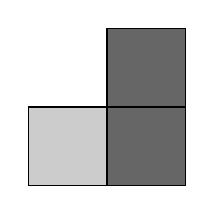
\begin{tikzpicture}
      \draw[fill=black!20] (0,0) grid (1,1) rectangle (0,0);
      \draw[fill=black!60] (1,0) grid (2,2) rectangle (1,0);
    \end{tikzpicture}
  \end{center}

\item You must have a expedition piece in the \textbf{lower left corner}.
\item You may not have any breaks in your path. It must be an \textbf{unbroken
    collection} of adjacent pieces.
\end{enumerate}

You may notice several Mobimon inhabiting the Expedition Zone! These Mobimon are
represented by \textbf{numbers,} and each number is its \textbf{strength.} To
catch a Mobimon, you must

\begin{enumerate}
\item make sure your path goes over that Mobimon, and
\item a piece on that Mobimon must have \textbf{more squares than that Mobimon's
  strength}.
\end{enumerate}

Your score is the \textbf{sum of the strengths of the Mobimon you catch}. The
teams with the two highest scores get \textbf{Victory Points}! Good luck!

\phWorksheet{Expedition Zone Map}

\begin{center}
  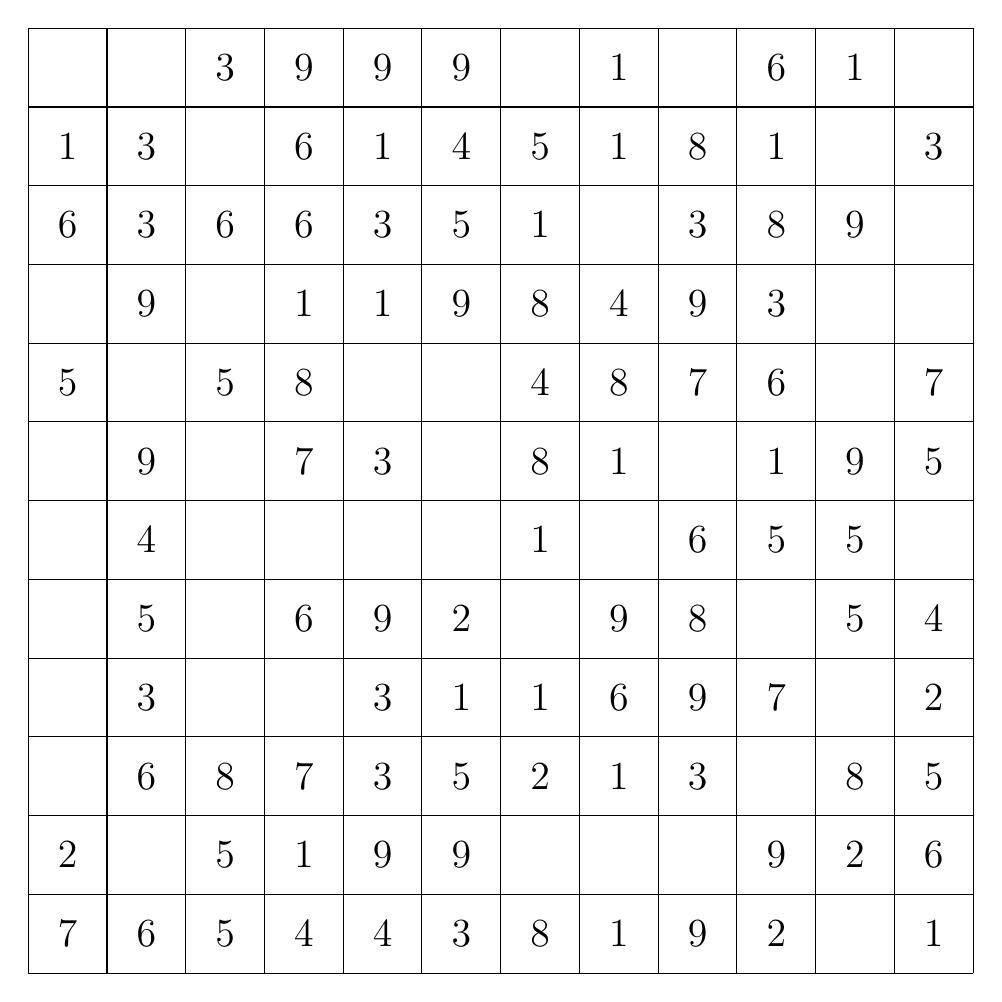
\begin{tikzpicture}
    \draw[step=10mm] (0,0) grid (12,12);

    % nodes - randomly generated by gridgenerator.py
    \tikzstyle{every node}=[font=\Large];
    % run the command:
    % > python gridgenerator.py
    % to generate a new set and copy/paste from gridgen.out (which is a text file
    % despite the unusual extension
    %there are exactly 500 points worth of mobimon
    \node at (5mm, 5mm){7};
    \node at (5mm, 15mm){2};
    \node at (5mm, 75mm){5};
    \node at (5mm, 95mm){6};
    \node at (5mm, 105mm){1};
    \node at (15mm, 5mm){6};
    \node at (15mm, 25mm){6};
    \node at (15mm, 35mm){3};
    \node at (15mm, 45mm){5};
    \node at (15mm, 55mm){4};
    \node at (15mm, 65mm){9};
    \node at (15mm, 85mm){9};
    \node at (15mm, 95mm){3};
    \node at (15mm, 105mm){3};
    \node at (25mm, 5mm){5};
    \node at (25mm, 15mm){5};
    \node at (25mm, 25mm){8};
    \node at (25mm, 75mm){5};
    \node at (25mm, 95mm){6};
    \node at (25mm, 115mm){3};
    \node at (35mm, 5mm){4};
    \node at (35mm, 15mm){1};
    \node at (35mm, 25mm){7};
    \node at (35mm, 45mm){6};
    \node at (35mm, 65mm){7};
    \node at (35mm, 75mm){8};
    \node at (35mm, 85mm){1};
    \node at (35mm, 95mm){6};
    \node at (35mm, 105mm){6};
    \node at (35mm, 115mm){9};
    \node at (45mm, 5mm){4};
    \node at (45mm, 15mm){9};
    \node at (45mm, 25mm){3};
    \node at (45mm, 35mm){3};
    \node at (45mm, 45mm){9};
    \node at (45mm, 65mm){3};
    \node at (45mm, 85mm){1};
    \node at (45mm, 95mm){3};
    \node at (45mm, 105mm){1};
    \node at (45mm, 115mm){9};
    \node at (55mm, 5mm){3};
    \node at (55mm, 15mm){9};
    \node at (55mm, 25mm){5};
    \node at (55mm, 35mm){1};
    \node at (55mm, 45mm){2};
    \node at (55mm, 85mm){9};
    \node at (55mm, 95mm){5};
    \node at (55mm, 105mm){4};
    \node at (55mm, 115mm){9};
    \node at (65mm, 5mm){8};
    \node at (65mm, 25mm){2};
    \node at (65mm, 35mm){1};
    \node at (65mm, 55mm){1};
    \node at (65mm, 65mm){8};
    \node at (65mm, 75mm){4};
    \node at (65mm, 85mm){8};
    \node at (65mm, 95mm){1};
    \node at (65mm, 105mm){5};
    \node at (75mm, 5mm){1};
    \node at (75mm, 25mm){1};
    \node at (75mm, 35mm){6};
    \node at (75mm, 45mm){9};
    \node at (75mm, 65mm){1};
    \node at (75mm, 75mm){8};
    \node at (75mm, 85mm){4};
    \node at (75mm, 105mm){1};
    \node at (75mm, 115mm){1};
    \node at (85mm, 5mm){9};
    \node at (85mm, 25mm){3};
    \node at (85mm, 35mm){9};
    \node at (85mm, 45mm){8};
    \node at (85mm, 55mm){6};
    \node at (85mm, 75mm){7};
    \node at (85mm, 85mm){9};
    \node at (85mm, 95mm){3};
    \node at (85mm, 105mm){8};
    \node at (95mm, 5mm){2};
    \node at (95mm, 15mm){9};
    \node at (95mm, 35mm){7};
    \node at (95mm, 55mm){5};
    \node at (95mm, 65mm){1};
    \node at (95mm, 75mm){6};
    \node at (95mm, 85mm){3};
    \node at (95mm, 95mm){8};
    \node at (95mm, 105mm){1};
    \node at (95mm, 115mm){6};
    \node at (105mm, 15mm){2};
    \node at (105mm, 25mm){8};
    \node at (105mm, 45mm){5};
    \node at (105mm, 55mm){5};
    \node at (105mm, 65mm){9};
    \node at (105mm, 95mm){9};
    \node at (105mm, 115mm){1};
    \node at (115mm, 5mm){1};
    \node at (115mm, 15mm){6};
    \node at (115mm, 25mm){5};
    \node at (115mm, 35mm){2};
    \node at (115mm, 45mm){4};
    \node at (115mm, 65mm){5};
    \node at (115mm, 75mm){7};
    \node at (115mm, 105mm){3};
  \end{tikzpicture}
\end{center}

\phWorksheet{Path Pieces}

\begin{center}
  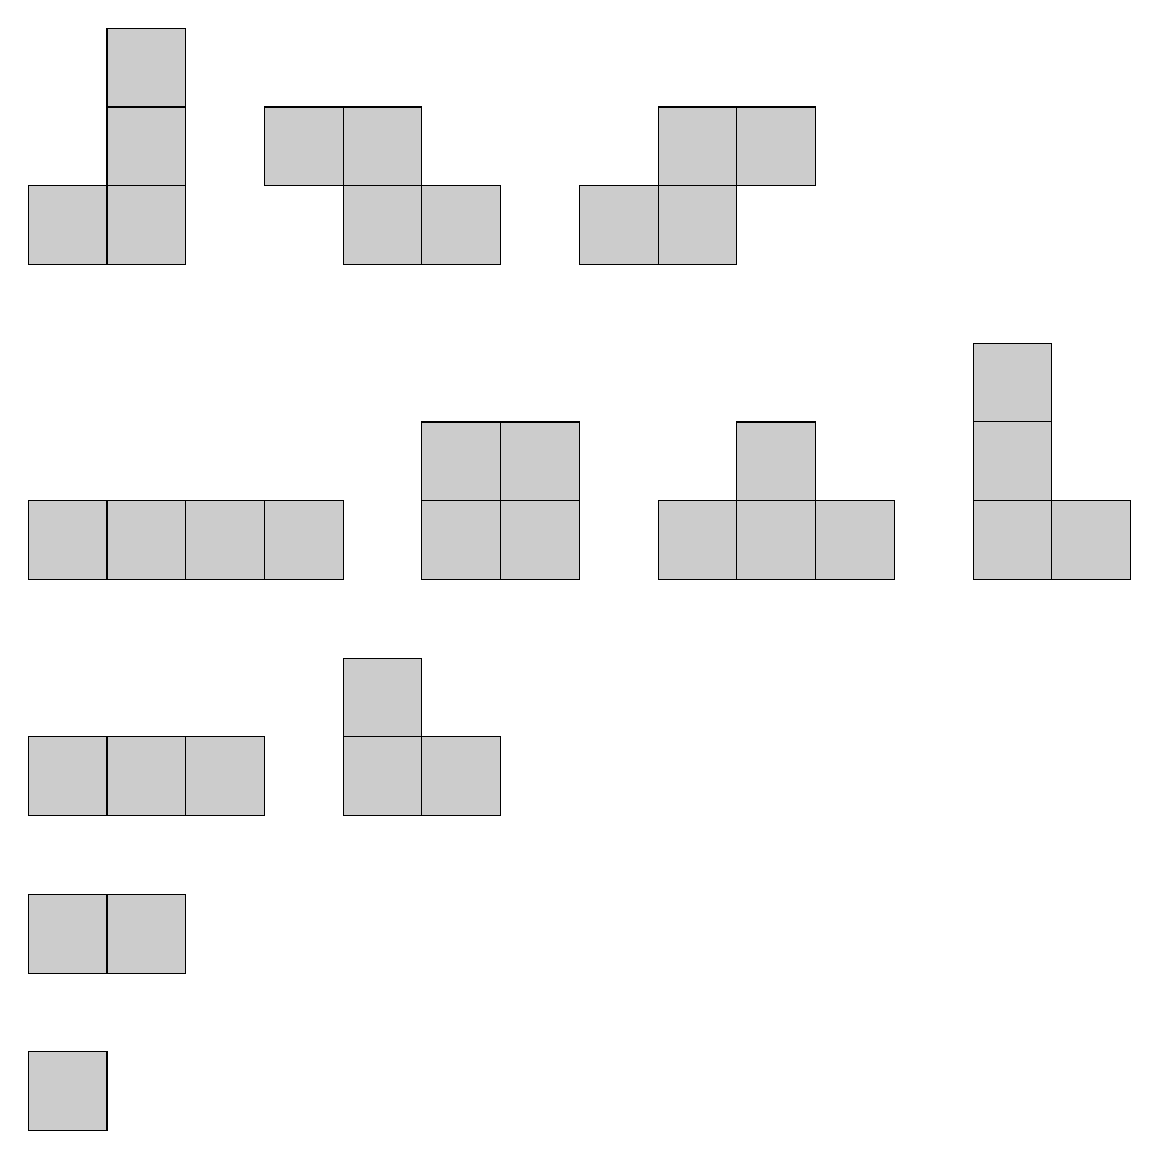
\begin{tikzpicture}
    % trailing rectangle is needed for filling with color
    % monomino
    \draw[step=10mm, fill=black!20] (0, -2) grid (1,-1) rectangle (0,-2);

    % domino
    \draw[step=10mm, fill=black!20] (0,0) grid (2,1) rectangle (0,0);

    % trominoes
    %% I
    \draw[step=10mm, fill=black!20] (0,2) grid (3,3) rectangle (0,2);
    %% L
    \draw[step=10mm, fill=black!20] (4,2) grid (6,3) rectangle (4,2);
    \draw[step=10mm, fill=black!20] (4,3) grid (5,4) rectangle (4,3);

    % tetraminoes
    %% I
    \draw[step=10mm, fill=black!20] (0,5) grid (4,6) rectangle (0,5);
    %% O
    \draw[step=10mm, fill=black!20] (5,5) grid (7,7) rectangle (5,5);
    %% T
    \draw[step=10mm, fill=black!20] (8,5) grid (11,6) rectangle (8,5);
    \draw[step=10mm, fill=black!20] (9,6) grid (10,7) rectangle (9,6);
    %% L
    \draw[step=10mm, fill=black!20] (12,5) grid (13,8) rectangle (12,5);
    \draw[step=10mm, fill=black!20] (13,5) grid (14,6) rectangle (13,5);
    %% J
    \draw[step=10mm, fill=black!20] (0,9) grid (2,10) rectangle (0,9);
    \draw[step=10mm, fill=black!20] (1,10) grid (2,12) rectangle (1,10);
    %% Z
    \draw[step=10mm, fill=black!20] (3,10) grid (5,11) rectangle (3,10);
    \draw[step=10mm, fill=black!20] (4,9) grid (6,10) rectangle (4,9);
    %% S
    \draw[step=10mm, fill=black!20] (7,9) grid (9,10) rectangle (7,9);
    \draw[step=10mm, fill=black!20] (8,10) grid (10,11) rectangle (8,10);
  \end{tikzpicture}
\end{center}

% Include below for aucTeX integration
%%% Local Variables:
%%% mode: latex
%%% TeX-master: "../mapp-challenge-18-game-book"
%%% End:
